\documentclass[titlepage,a4paper,12pt]{ltjsreport}

\usepackage{luatexja}
\usepackage{amsmath,amsfonts}
\usepackage{amsthm}
\usepackage{bm}
\usepackage[dvipdfmx]{graphicx}
\usepackage{color}
\usepackage{here}
\usepackage{caption}
\usepackage{url}
\usepackage{listings}
\usepackage{abstract}
\usepackage{multicol}
\usepackage{geometry}
\usepackage{here}

\lstset{
    basicstyle={\ttfamily},
    identifierstyle={\small},
    commentstyle={\small},
    keywordstyle={\small\bfseries},
    ndkeywordstyle={\small},
    stringstyle={\small\ttfamily},
    frame={tb},
    breaklines=true,
    columns=fixed,
    basewidth=0.465em,
    numbers=left,
    numberstyle={\scriptsize},
    lineskip=-0.5ex
}


\begin{document}

\leftline{課題1 要求記述}
\rightline{256E0143
三留 慎太郎}

\begin{enumerate}
    \item 概要 \mbox{}\\
    javaプログラム全体のLOC,クラス毎のLOC,クラス毎のメソッド数を数える。\\


    \item 詳細\mbox{}\\
    プログラム全体の規模を表す数とそれぞれのクラスの名前とクラス規模(インポートやパッケージ宣言を含む)とメソッド数を数える。\\
    プログラムはコーディング標準に準じて記述する。\\
    プログラム全体,クラス毎のLOCはカウンティング標準に準じて数える。\\


    表示する項目は、プログラム番号,クラス名,メソッド数,クラス規模,合計規模であり、各数字は整数で表示する。

    \item 入力\mbox{}\\
    
    \begin{itemize}
        \item javaファイルの入力:すべてのファイルを配置したディレクトリを指定して1ファイルずつファイル入力。
        \item ディレクトリ名:課題1,課題2など課題+プログラム番号とする
        \item 入力ファイル:コーディング標準に従って書かれたjavaファイル。
        
        \item 実行時の入力:コマンドラインに以下の形式で入力\\
         java プログラム名 課題+プログラム番号
        \item 実行時入力例:java Program2 課題2

    \end{itemize}


    \item 出力\mbox{}\\
    \begin{itemize}
        \item 出力方法:csvファイル出力。名前はoutput.csv。
        \item 出力する値:プログラム番号,クラス名,メソッド数,クラス規模,合計規模
        \item 精度:すべて整数で表示する
        \item 出力例:図\ref{out_example}のようにoutput.csvという名前で表として出力する。図はcsvファイルをexcelを用いて表示したもの。
        
        \begin{figure}[h]
            \centering
            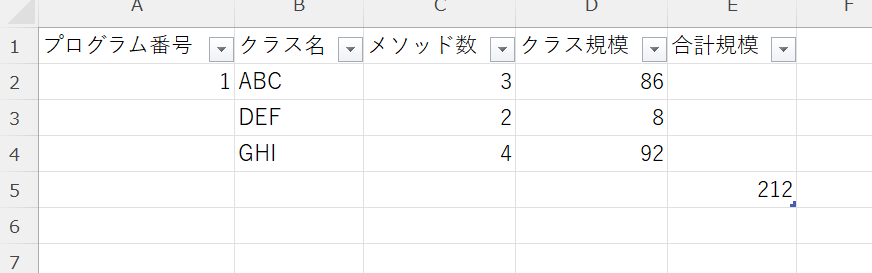
\includegraphics[width=0.4\textwidth]{../picture/課題2/out_example.png}
            \caption{出力例}
            \label{out_example}
        \end{figure}

    \end{itemize}

    \item 実行方法\mbox{}\\
    コマンドラインに\\
     java Program2 input\\
    と入力して実行する。
    \item テスト\mbox{}\\
    課題1で作成したプログラムと今回作成するプログラム自身を用いてそれぞれテストを行う。
    プログラム番号,クラス名,メソッド数,クラス規模,合計規模が正しくcsvファイルで出力されることを確認する。\\


    テスト1期待値:図\ref{out_kitai}のように課題1のプログラム番号,クラス名,メソッド数,クラス規模,合計規模をcsvファイルで出力する。
        
    \begin{figure}[h]
        \centering
        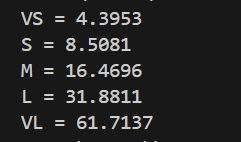
\includegraphics[width=0.4\textwidth]{../picture/課題2/kitaiti1.png}
        \caption{期待値}
        \label{out_kitai}
    \end{figure}

    今回作成するプログラムについても同様にコンパイル後、規模を求めテストを行う。

\end{enumerate}



\end{document}